\pdfoutput=1
\documentclass[11pt]{article}
% Remove the "review" option to generate the final version.
\usepackage{ACL2023}
\usepackage{times}
\usepackage{latexsym}
\usepackage[T1]{fontenc}
\usepackage[utf8]{inputenc}
\usepackage{microtype}
\usepackage{inconsolata}
\usepackage{pdflscape}
\usepackage{booktabs}
\usepackage{longtable}
\usepackage{graphicx}
\usepackage{subcaption}
\usepackage{dblfloatfix}

% Centered fixed width column type
\usepackage{array}
\newcolumntype{x}[1]{>{\centering\let\newline\\\arraybackslash\hspace{0pt}}m{#1}}

% Set math text size
\DeclareMathSizes{8}{8}{8}{8}

\title{The Practicality of Prompt Engineering}

\author{Isaac Liu\thanks{~~Feedback from David Bamman, Kent Chang, Morris Chang, Kenan Carames, Mayank Bhushan, Ankita Shanbhag, and Wenjing Lin was much appreciated. Mingyu Yuan's advice encouraging the implementation of an objective measure of passage coherence was particularly helpful.}
\\
  University of California, Berkeley \\
  \texttt{ijyliu@berkeley.edu}}

% stattotex loading
\newcommand{\pAtlOneHumanEqAggPct}{76.5\%}
\newcommand{\simProbAgmtCmplStr}{21.84\%}


\begin{document}
\maketitle

\begin{abstract}
  This paper examines the practicality of prompt engineering in improving the performance of Large Language Models (LLMs). Through empirical analysis, I evaluate the trade-offs between costs and benefits of prompting using novel metrics. Different prompting methods are assessed using standardized tasks and both state-of-the-art and older models.
\end{abstract}

\section*{Introduction}

Prompt engineering, the practice of developing specialized prompts and queries to improve the accuracy of Large Language Models, is a prominent topic of interest in the NLP community, and among the general public. The practice is believed to allow for improvements in LLM performance in a variety of domains without investment in underlying training \cite{martineau_what_2021}. It is not, however, without its critics. Some commentators believe that the practice will become irrelevant as models grow larger and more powerful, becoming more capable of directly interpreting a user's intent without error \cite{ethan_mollick_emollick_i_2023}. Others question the need for specialized professionals or training to attain minimal improvements which are often not repeatable across contexts \cite{shackell_prompt_2023, acar_ai_2023}. 

Despite such controversy, it is difficult to find empirical analyses of the tradeoff between costs and accuracy benefits associated with advanced prompting. Papers introducing new prompting techniques often only include performance benchmarks concerning the techniques' efficacy, typically within a limited domain. Some authors briefly mention problems associated with involved prompting, such as the human time and effort induced by increased complexity and limitations on creativity and randomness \cite{wu_ai_2022}, and others suggest the automation of prompting to avoid some of these costs \cite{diao_active_2023}. It is known that token costs, degradation of quality with increased prompt context lengths, and the uncertain nature of accuracy gains are all important practical considerations \cite{gao_prompt_2023}. However, the extent of these issues for various techniques, so as to enable standardized comparison between them and with a control baseline (no special prompting), has not been (to my knowledge) quantified.

The quality, length, and complexity of LLM responses have been analyzed within several individual task and technique domains. Some research with GPT-3 series models on math and non-math reasoning tasks suggests the addition of length and complexity through the introduction of extra reasoning steps for both input prompts and output responses improves performance when using chain-of-thought prompting techniques \cite{fu_complexity-based_2023}. Effects are on the magnitude of several points of accuracy per added step, with generally low costs as long as prompt examples are selected carefully. Uniform improvements from complex chain-of-thought prompting are not fully accepted in the literature, however - other work has noted a tendency for the method to lead to worse performance on simple questions \cite{shum_automatic_2023}.

Complexity has also been studied within the context of prompting for summarization and story generation tasks. The Chain of Density prompting technique seeks to optimize the named entity density of LLM-generated summaries through choice from a series of repeated, increasingly dense iterations \cite{adams_sparse_2023}. Human preferences tend to align with 0.1 - 0.15 named entities per token, a point near the middle of the usual sequence of generations, demonstrating the existence of a tradeoff between informativeness and clarity. At the same time, other work has shown is difficult to control language model output complexity, meaning that the choice of specific techniques is important. Research demonstrates current models are not yet able to achieve compliance with desired readability instructions for the tasks of story generation, simplification, and summarization, though a small amount of improvement is achievable through careful prompt word choice and the use of few-shot examples \cite{pu_chatgpt_2023, imperial_flesch_2023}.

This paper uses several metrics to evaluate the benefits and drawbacks of prompt engineering methods systematically, and analyzes the tradeoffs inherent in their application to standardized data. Such an assessment is valuable on several dimensions. Beyond quantifiably testing the practicality of prompt engineering as a whole, it can be used to compare the performance of different approaches, useful in a world where so many competing techniques are available. I also provide a newly constructed dataset summarizing the wide variety of existing techniques and data on their popularity as measured by Semantic Scholar citations, which may be useful for future surveys of the field. Next, I offer a new look at these prompting methods in a period long after their introduction. The current environment is one in which far greater capabilities are native to underlying foundation models. Finally, I introduce and adapt some useful measures of costs and complexity, such as the ratio of interaction length with prompting to the length of an accepted human-generated answer, to the challenge of LLM evaluation.

\section*{Data}

To evaluate performance, I attempt to use tasks that are general-purpose, close to real-world applications, and standardized in the literature. To this end, I selected the GSM8K dataset, a collection of elementary-level math word problems \cite{cobbe_training_2021}, and a creative writing task involving the generation of a coherent two-paragraph passage with random, predetermined ending sentences for each paragraph. The original creative writing task in \citealp{yao_tree_2023} uses four paragraphs and sentences, but this is too difficult for older models and for the manual production of good answer demonstrations - I simply take the first two sentences for each original question. 

These tasks carry several key benefits. They cover both the mathematical and linguistic domains - two types of tasks that form the foundation of the standardized testing of humans. GSM8K is studied in the majority of the papers introducing techniques used in this paper and is among the most common datasets used in the far larger list of papers I initially surveyed. Text and story generation is a widespread foundational task in NLP. Importantly, these sets of tasks are known to be free of data contamination. The GSM8K test set has been intentionally withheld from the training of OpenAI's models \cite{openai_gpt-4_2023}. The creative writing task was released only in 2023, and the code and data provided with the associated paper includes only questions and not LLM responses. \footnote{It is also relatively simple to find random sentence generators online (such as \url{https://www.thewordfinder.com/random-sentence-generator/}), which would work for this task - at the cost of comparability with the results of \cite{yao_tree_2023}. In any case, the 2-sentence task represents a modification of the original, and the test overall makes use of subjective human evaluations of the coherence of generated stories, limiting comparisons anyway - so perhaps testing the task on more truly novel pairings is a promising direction for future work.}

I perform the analysis on one cutting-edge model and one older model from closer to the time that these techniques were introduced. This provides a picture of the changing costs and benefits of advanced prompting, a trend that may even be extrapolated into the future if current LLM scaling laws continue to hold. As the most widely used models and the ones behind much original work in the field, I select two models from the OpenAI series: GPT-4 (June 13th, 2023 version: 'gpt-4-0613') and text-davinci-003. All conversations were conducted programatically via the OpenAI API.

%To the extent possible, I report accuracy scores on the domain dataset as they are in the original paper introducing each technique. It is possible to use any prompts, LLM responses, and correct responses provided along with original papers to calculate other simple metrics such as response lengths and complexity. However, some metrics (time taken, human assessments of complexity) require my own evaluations.
% Note - this can be a part of any accuracy discussions
% It might be interesting to see if the creative writing coherency scores are higher in my results using two sentences relative to the Yao results using four sentences.

\section*{Prompting Methods Assessed}

The following methods were selected based on their popularity (see Appendix Section \ref{sec:popularity}) and ease of implementation. A full list of all prompts for each task can be found in Appendix Section \ref{sec:prompts}.

\begin{itemize}
  \item Zero-Shot Control Baseline/Direct Prompting: This method consists of just providing the question/task directly.
  \item Zero-Shot Chain of Thought Prompting (Original): Initial advances in chain of thought prompting to improve reasoning were achieved by simply including the following before the question/task: "Let's think step by step." \cite{kojima_large_2023} For the creative writing task, the prompt following the question/task is adapted to: "Plan step-by-step before writing the passage." \footnote{In initial experiments, this modification was found necessary to elicit any sort of step-by-step behavior from the model.}
  \item Zero-Shot Chain of Thought Prompting (Automatic Prompt Engineer): Automated testing has indicated that an optimal zero-shot Chain of Thought prompt is "Let's work this out in a step by step way to be sure we have the right answer." \cite{zhou_large_2022} For the creative writing task, the prompt following the question/task is adapted to: "Plan step-by-step before writing the passage to be sure we have a correct and coherent answer." \footnote{Again, in initial experiments, this modification was found necessary to elicit any sort of step-by-step behavior from the model.}
  \item Tree of Thought Prompting: The language model traverses a tree of decisions - choosing among multiple steps or ideas it has generated to arrive at a conclusion. Backtracking is possible. \cite{yao_tree_2023}
  \item Self-Refine Prompting: The model produces an initial response, then is prompted for feedback which it uses for refinement. \cite{madaan_self-refine_2023}
  \item Least-to-most Prompting: The model is given few-shot examples that demonstrate how to first break down the task into smaller and simpler subproblems, then solve them sequentially. \cite{zhou_least--most_2023}
  \item Few-Shot Prompting: The prompter provides a few examples of successfully answered questions or tasks before the main question/task.
  \item Few-Shot Chain-of-Thought Prompting: The model is provided worked examples of answers in which the reasoning steps are written out. \cite{wei_chain--thought_nodate} Note, however, that such steps are not explicitly planned out or mentioned, as is the case in least-to-most prompting.
\end{itemize}

\section*{Analyses}

In this section I will discuss each metric's construction, report the results with a graph or table, and discuss the results as well as any connections to the literature.

I provide accuracy scores as well as summary statistics (mean, standard deviation) of the metrics listed below for each prompting method by model by question/task type. Statistical inference is uncommon in the prompting literature - most papers simply report accuracy. \footnote{Effect sizes and sample sizes are usually sufficiently large to merit confidence in the statistical significance of results. All paired t-tests comparing prompting methods and human responses were significant in the one paper I did find with inference, \citealp{pu_chatgpt_2023}.} However, in this work, I do check for significant differences in metrics between prompting methods, reporting at the 95\% level. For GSM8K accuracy scores I perform McNemar's test comparing each method to the direct prompting baseline. \footnote{The same questions are administered for each prompting method, so there is dependence that this paired test accounts for.} For sample means of creative writing scores and other statistics, I perform paired t-tests. \footnote{One other metric remains - the token cost of accuracy or change in accuracy divided by change in tokens for each method versus direct prompting. Bootstrapping confidence intervals for this value seems possible, but the dependent nature of the data poses challenges.}

\subsection*{Quality and Accuracy}

I report:

For GSM8K problems:
\begin{itemize}
  \item Correct/Incorrect accuracy at the point a technique has been fully implemented (the end of the tree of thought or after all self-refinement, etc.)
\end{itemize}

For Creative Writing:
\begin{itemize}
  \item Human assessment of coherence (on a scale of 1 to 10, 1 being incoherent and 10 being very coherent). GPT-4 is known to be capable of producing scalar scores useful for this task \cite{yao_tree_2023}, so I also collect its evaluations as an additional opinion (see Appendix Section \ref{sec:evaluating_creative_writing}). I report human scores, GPT-4 scores, the average of them, and Krippendorff's alpha. I also collect data on whether or not the task constraints were followed (whether ending sentences exactly match those specified), and additionally report scores when the lowest possible rating of 1 is assigned to cases where the rules are broken. \footnote{I additionally tried to use GPT-4 to assess adherence to the original instructions - to check if the exact sentences specified in the prompt were used. In my initial experiments - in contrast to \citealp{yao_tree_2023} - I found that GPT-4 was not able to do this, repeatedly missing deviations of one or a few words, even when told to carefully perform the check in a step-by-step manner!}
\end{itemize}

%\begin{tabular}{x{0.75cm}|x{1.5cm}|x{0.75cm}|x{0.75cm}|x{0.75cm}|x{0.75cm}|x{0.75cm}|x{0.75cm}|x{0.75cm}|x{0.75cm}|x{0.75cm}}
\toprule
\hline
Task & Metric & Model & Manual Few-Shot (May 2020) & Manual CoT (Jan 2022) & Least-to-Most (May 2022) & Zero-Shot CoT (May 2022) & APE Zero-Shot CoT (Nov 2022) & Self-Refine (Mar 2023) & Tree-of-Thought (May 2023) & Direct Prompting \\
\hline
\midrule
GSM8K & Accuracy & Text-Davinci-003 & 0.18 & 0.6* & 0.67* & 0.62* & 0.49* & 0.2 & 0.23 & 0.23 \\
\hline
 &  & GPT-4 & 0.49* & 0.93* & 0.95* & 0.95* & 0.93* & 0.89* & 0.4* & 0.73 \\
\hline
Creative Writing & Average Inter-Sentence Cosine Similarity & Text-Davinci-003 & 0.364 (0.004) & 0.345 (0.004) & 0.357 (0.003) & 0.366 (0.006) & 0.382* (0.006) & 0.369 (0.004) & 0.357 (0.009) & 0.363 (0.004) \\
\hline
 &  & GPT-4 & 0.346 (0.004) & 0.35* (0.004) & 0.341 (0.004) & 0.347* (0.003) & 0.35* (0.004) & 0.356* (0.004) & 0.351* (0.004) & 0.333 (0.002) \\
\hline
 & Average Inter-Paragraph Cosine Similarity & Text-Davinci-003 & 0.476* (0.027) & 0.479* (0.026) & 0.48* (0.026) & 0.41* (0.037) & 0.42* (0.037) & 0.366 (0.032) & 0.43 (0.049) & 0.359 (0.032) \\
\hline
 &  & GPT-4 & 0.386* (0.021) & 0.422 (0.021) & 0.422 (0.023) & 0.465* (0.023) & 0.464* (0.022) & 0.412 (0.026) & 0.447 (0.021) & 0.42 (0.025) \\
\hline
 & Average Inter-Sentence Cosine Similarity (Compliance Adjusted) & Text-Davinci-003 & 0.363 (0.004) & 0.351 (0.004) & 0.369 (0.004) & 0.386 (0.006) & 0.391* (0.005) & 0.393 (0.003) & 0.397 (0.011) & 0.368 (0.005) \\
\hline
 &  & GPT-4 & 0.349 (0.003) & 0.355* (0.005) & 0.35* (0.004) & 0.344 (0.003) & 0.356 (0.004) & 0.351 (0.004) & 0.348 (0.004) & 0.334 (0.002) \\
\hline
 & Average Inter-Paragraph Cosine Similarity (Compliance Adjusted) & Text-Davinci-003 & 0.433* (0.031) & 0.401 (0.037) & 0.414 (0.028) & 0.357 (0.033) & 0.389 (0.034) & 0.34 (0.042) & 0.224 (0.02) & 0.371 (0.032) \\
\hline
 &  & GPT-4 & 0.366* (0.024) & 0.423 (0.022) & 0.404 (0.025) & 0.463* (0.024) & 0.449 (0.025) & 0.398 (0.025) & 0.455 (0.02) & 0.42 (0.025) \\
\hline
 & Compliance & Text-Davinci-003 & 0.43 & 0.19* & 0.25* & 0.43 & 0.44 & 0.32* & 0.04* & 0.5 \\
\hline
 &  & GPT-4 & 0.63 & 0.51 & 0.52 & 0.57 & 0.56 & 0.48 & 0.26* & 0.56 \\
\hline
\bottomrule
\end{tabular}


Grader coherence scores are inherently noisy, as noted in \citealp{yao_tree_2023}, but I take several measures to ameliorate this problem. First, I limit reported results to information concerning which method was preferred for each model and selection of ending sentences. This limits demands on the data to only the ordinal ranking of methods. Second, I check the consistency of my methodology and results by soliciting a secondary opinion. I fine-tuned GPT-3.5 to learn my methodology for grading passage coherence - a difficult task, given the difficult nature of coherence as a concept and the wide variety of LLM responses and associated formats resulting from different models and methods. I created two fine-tuned models, each trained and validated on a randomly selected 50\% fold of responses (stratified by method) and human coherence scores and deployed on the other 50\% fold. The results demonstrate the consistency of human preferences. For \pAtlOneHumanEqAggPct~of model-sentence pairings, at least human and automated scores agree on at least one of the methods as among the top-preferred. Simulations using empirical probabilities of scores under independence indicate that this would occur in only \simProbAgmtCmplStr~of cases by chance.

Figure \ref{fig:cw_preference_plot_ca} shows the number of conversations where each method was one of the most preferred.

For my main results, however, I introduce more objective measures of passage coherence that give a good sense of the concept on various levels. To assess local coherence between sentences, I compute the average cosine similarity between consecutive sentence-level BERT embeddings (all-distilroberta-v1). For a more global measure, I compute average embeddings for each paragraph of the LLM response and compute the average cosine similarity between these paragraph embeddings for consecutive paragraphs. \footnote{Other structural methods for assessing global coherence were considered, but not implemented due to their limited additional value and overall feasibility for short, 2-paragraph passages.}

% Potentially add math here

\begin{centering}

  %\onecolumn

  % \begin{table*}
  %   \caption{Human-Preferred Method by Model - Creative Writing Coherence}
  %   \centering
  %   \begin{tabular}{c c c}
\toprule
Model & Method & Conversations as a Top Method \\
\midrule
Text-Davinci-003 & Manual Few-Shot & 32 \\
 & Direct Prompting & 24 \\
 & Least-to-Most & 21 \\
 & Self-Refine & 17 \\
 & Manual CoT & 16 \\
 & Zero-Shot CoT & 16 \\
 & APE Zero-Shot CoT & 13 \\
 & Tree-of-Thought & 7 \\
GPT-4 & Self-Refine & 31 \\
 & Zero-Shot CoT & 27 \\
 & Manual Few-Shot & 26 \\
 & Direct Prompting & 24 \\
 & Manual CoT & 22 \\
 & Least-to-Most & 17 \\
 & APE Zero-Shot CoT & 14 \\
 & Tree-of-Thought & 6 \\
\bottomrule
\end{tabular}
  
  % \end{table*}
  
  % \begin{table*}
  %   \caption{Human-Preferred Method by Model - Creative Writing Coherence - Adjust for Non-Compliance}
  %   \centering
  %   \begin{tabular}{c c c}
\toprule
Model & Method & Conversations as a Top Method \\
\midrule
Text-Davinci-003 & Direct Prompting & 35 \\
 & Manual Few-Shot & 34 \\
 & APE Zero-Shot CoT & 31 \\
 & Self-Refine & 27 \\
 & Zero-Shot CoT & 27 \\
 & Least-to-Most & 26 \\
 & Manual CoT & 22 \\
 & Tree-of-Thought & 14 \\
GPT-4 & Zero-Shot CoT & 28 \\
 & Manual Few-Shot & 26 \\
 & Direct Prompting & 25 \\
 & Self-Refine & 24 \\
 & APE Zero-Shot CoT & 22 \\
 & Least-to-Most & 20 \\
 & Manual CoT & 20 \\
 & Tree-of-Thought & 11 \\
\bottomrule
\end{tabular}
  
  % \end{table*}

  % \begin{figure*}
  %   \caption{Human-Preferred Method by Model - Creative Writing Coherence}
  %   \centering
  %   \includegraphics[width=\textwidth]{../Output/cw_preference_plot_coherence_1_incoherent_10_very_coherent_coherence_1_incoherent_10_very_coherent.png}
  % \end{figure*}

  \begin{figure*}
    \caption{Human-Preferred Method by Model - Creative Writing Coherence - Adjust for Non-Compliance}
    \centering
    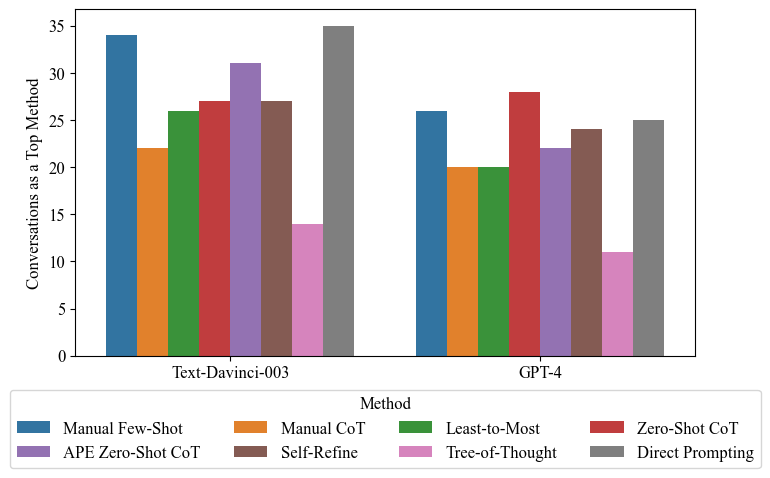
\includegraphics[width=\textwidth]{../Output/cw_preference_plot_coherence_1_incoherent_10_very_coherent_compliance_adjusted.png}
    \label{fig:cw_preference_plot_ca}
  \end{figure*}

  \begin{table*}
    \caption{Mean and Standard Deviation of Accuracy/Quality Scores}
    \centering
    \tiny
    \begin{tabular}{x{0.75cm}|x{1.5cm}|x{0.75cm}|x{0.75cm}|x{0.75cm}|x{0.75cm}|x{0.75cm}|x{0.75cm}|x{0.75cm}|x{0.75cm}|x{0.75cm}}
\toprule
\hline
Task & Metric & Model & Manual Few-Shot (May 2020) & Manual CoT (Jan 2022) & Least-to-Most (May 2022) & Zero-Shot CoT (May 2022) & APE Zero-Shot CoT (Nov 2022) & Self-Refine (Mar 2023) & Tree-of-Thought (May 2023) & Direct Prompting \\
\hline
\midrule
GSM8K & Accuracy & Text-Davinci-003 & 0.18 & 0.6* & 0.67* & 0.62* & 0.49* & 0.2 & 0.23 & 0.23 \\
\hline
 &  & GPT-4 & 0.49* & 0.93* & 0.95* & 0.95* & 0.93* & 0.89* & 0.4* & 0.73 \\
\hline
Creative Writing & Average Inter-Sentence Cosine Similarity & Text-Davinci-003 & 0.364 (0.004) & 0.345 (0.004) & 0.357 (0.003) & 0.366 (0.006) & 0.382* (0.006) & 0.369 (0.004) & 0.357 (0.009) & 0.363 (0.004) \\
\hline
 &  & GPT-4 & 0.346 (0.004) & 0.35* (0.004) & 0.341 (0.004) & 0.347* (0.003) & 0.35* (0.004) & 0.356* (0.004) & 0.351* (0.004) & 0.333 (0.002) \\
\hline
 & Average Inter-Paragraph Cosine Similarity & Text-Davinci-003 & 0.476* (0.027) & 0.479* (0.026) & 0.48* (0.026) & 0.41* (0.037) & 0.42* (0.037) & 0.366 (0.032) & 0.43 (0.049) & 0.359 (0.032) \\
\hline
 &  & GPT-4 & 0.386* (0.021) & 0.422 (0.021) & 0.422 (0.023) & 0.465* (0.023) & 0.464* (0.022) & 0.412 (0.026) & 0.447 (0.021) & 0.42 (0.025) \\
\hline
 & Average Inter-Sentence Cosine Similarity (Compliance Adjusted) & Text-Davinci-003 & 0.363 (0.004) & 0.351 (0.004) & 0.369 (0.004) & 0.386 (0.006) & 0.391* (0.005) & 0.393 (0.003) & 0.397 (0.011) & 0.368 (0.005) \\
\hline
 &  & GPT-4 & 0.349 (0.003) & 0.355* (0.005) & 0.35* (0.004) & 0.344 (0.003) & 0.356 (0.004) & 0.351 (0.004) & 0.348 (0.004) & 0.334 (0.002) \\
\hline
 & Average Inter-Paragraph Cosine Similarity (Compliance Adjusted) & Text-Davinci-003 & 0.433* (0.031) & 0.401 (0.037) & 0.414 (0.028) & 0.357 (0.033) & 0.389 (0.034) & 0.34 (0.042) & 0.224 (0.02) & 0.371 (0.032) \\
\hline
 &  & GPT-4 & 0.366* (0.024) & 0.423 (0.022) & 0.404 (0.025) & 0.463* (0.024) & 0.449 (0.025) & 0.398 (0.025) & 0.455 (0.02) & 0.42 (0.025) \\
\hline
 & Compliance & Text-Davinci-003 & 0.43 & 0.19* & 0.25* & 0.43 & 0.44 & 0.32* & 0.04* & 0.5 \\
\hline
 &  & GPT-4 & 0.63 & 0.51 & 0.52 & 0.57 & 0.56 & 0.48 & 0.26* & 0.56 \\
\hline
\bottomrule
\end{tabular}
  
    \label{tab:accuracy_quality}
    \newline \newline \footnotesize Stars indicate a significant difference from the direct prompting baseline from McNemar's test at the 95\% level for GSM8K accuracy scores and creative writing task compliance scores and paired t-tests at the 95\% level for all other metrics.
  \end{table*}

  %\clearpage

  %\twocolumn

\end{centering}

General Discussion:

Which methods perform the best, and are the differences significant?

Do larger/more modern models benefit more from prompt engineering, or are the techniques becoming obsolete? Earlier evidence demonstrated that gains from few-shot learning increased with scale - has this trend continued to hold? \cite{brown_language_2020} Are the most recent prompt engineering techniques (as measured by paper release/publication date) more powerful and useful?

Are improvements from a given method replicable across tasks? Are they replicable within tasks (what is the variance of the indicator for getting a question right or of coherency scores)?

\subsection*{Length and Complexity}

For length, I report:

\begin{itemize}
  \item Length of the entire interaction in tokens (using OpenAI's tiktoken tokenizer for the appropriate model)
  \item Length of all prompts (all input) in tokens
  \item Financial cost of the entire interaction using OpenAI's prices per 1,000 tokens (accounting for different input/output prices with GPT-4)
  \item Length of the entire interaction in tokens relative to the length of the task/question + a baseline answer. For GSM8K, the baselines are the provided (OpenAI) solution and the answer achieved via direct prompting. For the Creative Writing task, the baseline is the answer achieved via direct prompting. How much is prompt engineering stretching the interaction out? The ratio of engineered answer length to baseline lengths can be informative. \footnote{I report a ratio as a difference in token counts would be harder to interpret directly - though it could easily be calculated by the reader using the length metrics.}
  \item The change in accuracy (in percentage points, 0 to 100) or quality (coherence scale points) divided by the change in tokens (difference in token counts), between the prompt engineering technique and direct prompting. Is any stretching of output adding value/improving accuracy/quality?
  \begin{displaymath}
    \frac{AQ_{PE} - AQ_{B}}{Tokens_{PE} - Tokens_{B}}
  \end{displaymath}
\end{itemize}

%\onecolumn

\begin{table*}
  \caption{Mean and Standard Deviation of Length Metrics}
  \centering
  \tiny
  \begin{tabular}{x{0.75cm}|x{1.5cm}|x{0.75cm}|x{0.75cm}|x{0.75cm}|x{0.75cm}|x{0.75cm}|x{0.75cm}|x{0.75cm}|x{0.75cm}|x{0.75cm}}
\toprule
\hline
Task & Metric & Model & Manual Few-Shot & Manual CoT & Least-to-Most & Zero-Shot CoT & APE Zero-Shot CoT & Self-Refine & Tree-of-Thought & Direct Prompting \\
\hline
\midrule
GSM8K & Conversation Length & Text-Davinci-003 & 533.94* (447.835) & 722.7* (1258.051) & 272.27* (2482.462) & 166.02* (2228.222) & 181.76* (3024.467) & 125.99* (1308.636) & 248.8* (13512.99) & 87.06 (1765.956) \\
\hline
 &  & GPT-4 & 579.69* (442.519) & 850.04* (2596.928) & 332.36* (3386.758) & 223.88* (3498.47) & 243.93* (3466.712) & 344.86* (13512.425) & 764.72* (97569.577) & 146.69 (6327.044) \\
\hline
 & Input Length & Text-Davinci-003 & 531.48* (442.818) & 655.48* (442.818) & 158.48* (442.818) & 67.48* (442.818) & 80.48* (442.818) & 99.48* (442.818) & 137.68* (6009.755) & 59.48 (442.818) \\
\hline
 &  & GPT-4 & 567.5* (441.505) & 741.5* (441.505) & 181.5* (441.505) & 80.5* (441.505) & 93.5* (441.505) & 167.7* (1460.394) & 407.42* (23824.933) & 72.5 (441.505) \\
\hline
 & Conversation Cost & Text-Davinci-003 & 0.011* (0.0) & 0.014* (0.0) & 0.005* (0.0) & 0.003* (0.0) & 0.004* (0.0) & 0.003* (0.0) & 0.005* (0.0) & 0.002 (0.0) \\
\hline
 &  & GPT-4 & 0.018* (0.0) & 0.029* (0.0) & 0.014* (0.0) & 0.011* (0.0) & 0.012* (0.0) & 0.016* (0.0) & 0.034* (0.0) & 0.007 (0.0) \\
\hline
Creative Writing & Conversation Length & Text-Davinci-003 & 695.41* (993.335) & 960.51* (1328.374) & 1025.02* (1194.323) & 256.53* (2207.343) & 274.04* (3433.13) & 382.19* (20049.347) & 916.81* (24662.277) & 200.41 (934.244) \\
\hline
 &  & GPT-4 & 751.04* (1244.099) & 968.75* (3092.634) & 1091.41* (2189.658) & 459.98* (2462.969) & 470.72* (2815.032) & 520.06* (44192.441) & 1325.17* (25140.971) & 337.33 (1913.031) \\
\hline
 & Input Length & Text-Davinci-003 & 504.49* (59.242) & 683.49* (59.242) & 736.49* (59.242) & 63.49* (59.242) & 73.49* (59.242) & 140.48* (1450.697) & 209.49* (59.242) & 52.49 (59.242) \\
\hline
 &  & GPT-4 & 522.21* (56.127) & 701.89* (55.553) & 754.89* (55.553) & 75.21* (56.127) & 84.89* (55.553) & 160.37* (1924.013) & 264.89* (55.553) & 65.89 (55.553) \\
\hline
 & Conversation Cost & Text-Davinci-003 & 0.014* (0.0) & 0.019* (0.0) & 0.021* (0.0) & 0.005* (0.0) & 0.005* (0.0) & 0.008* (0.0) & 0.018* (0.0) & 0.004 (0.0) \\
\hline
 &  & GPT-4 & 0.029* (0.0) & 0.037* (0.0) & 0.043* (0.0) & 0.025* (0.0) & 0.026* (0.0) & 0.026* (0.0) & 0.072* (0.0) & 0.018 (0.0) \\
\hline
\bottomrule
\end{tabular}
  
  \label{tab:avg_length_metrics_pivot}
  \newline \newline \footnotesize Stars indicate a significant difference from the direct prompting baseline from paired t-tests at the 95\% level.
\end{table*}

\begin{figure*}
  \caption{Average Length vs. Provided Length - GSM8K}
  \centering
  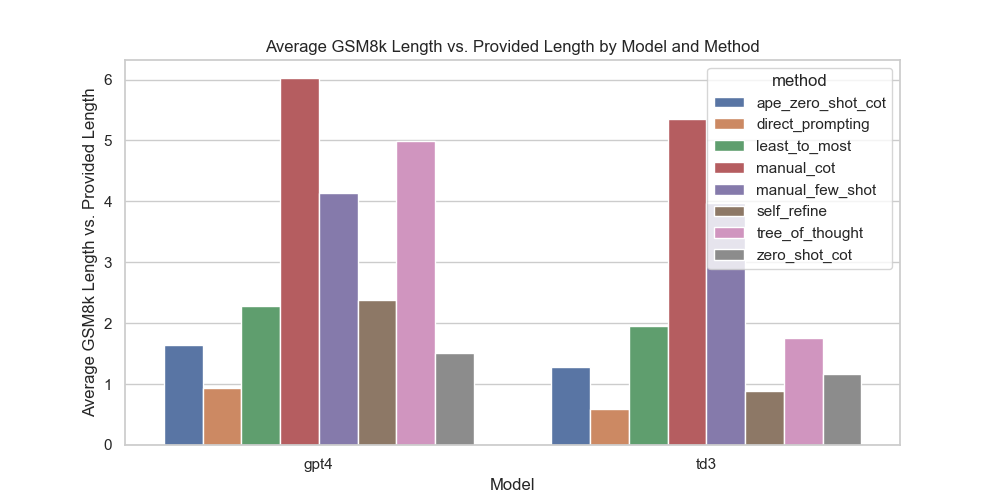
\includegraphics[width=\textwidth]{../Output/gsm8k_length_vs_provided_means.png}
  \label{fig:gsm8k_len_v_prov}
\end{figure*}

\begin{figure*}
  \caption{Average Length vs. Direct Prompting Length}
  \begin{subfigure}[h]{0.4925\textwidth}
      \centering
      \subcaption{GSM8K}
      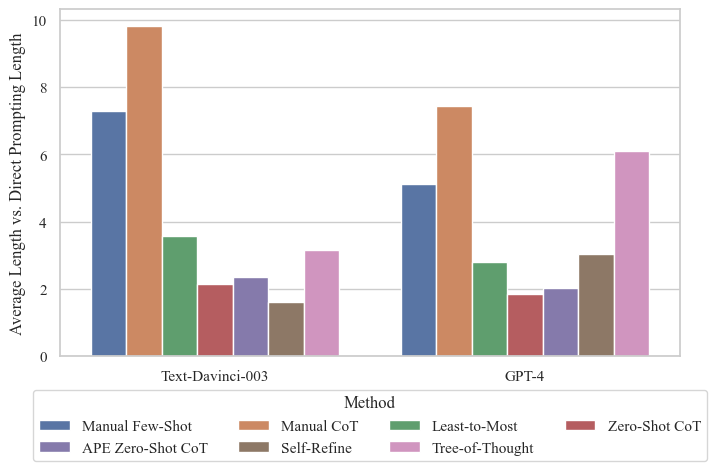
\includegraphics[width=0.95\hsize]{../Output/gsm8k_length_vs_direct_prompting_means.png} 
  \end{subfigure}
  %\hfill
  \begin{subfigure}[h]{0.4925\textwidth}
      \centering
      \subcaption{Creative Writing}
      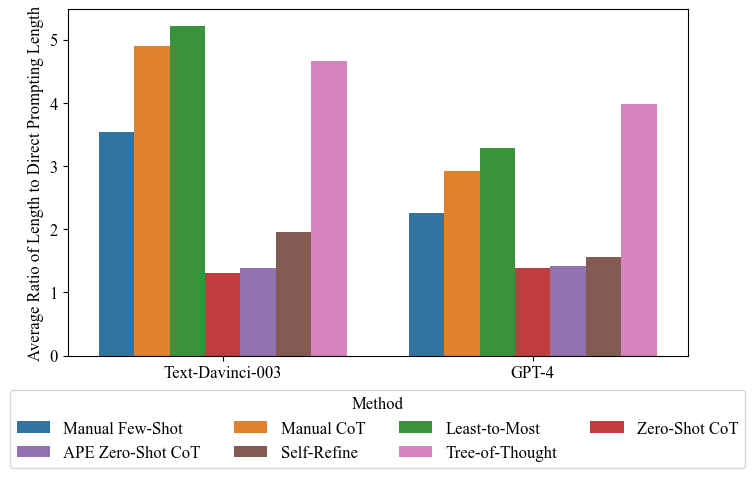
\includegraphics[width=0.95\hsize]{../Output/cw_length_vs_direct_prompting_means.png}
  \end{subfigure}
  \hfill
\end{figure*}

\begin{figure*}
  \caption{Gains v. Direct Prompting}
  \begin{subfigure}[h]{0.4925\textwidth}
      \centering
      \subcaption{GSM8K}
      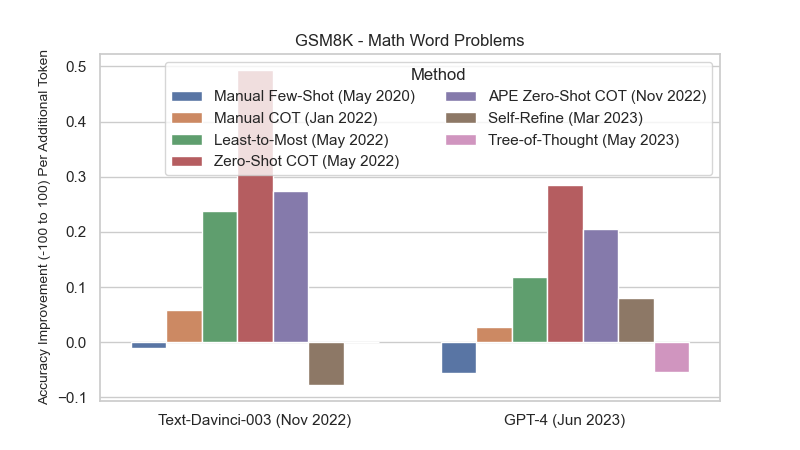
\includegraphics[width=0.95\hsize]{../Output/gsm8k_change_in_accuracy_quality_per_change_in_conversation_length_sorted_by_technique_age.png} 
  \end{subfigure}
  %\hfill
  \begin{subfigure}[h]{0.4925\textwidth}
      \centering
      \subcaption{Creative Writing}
      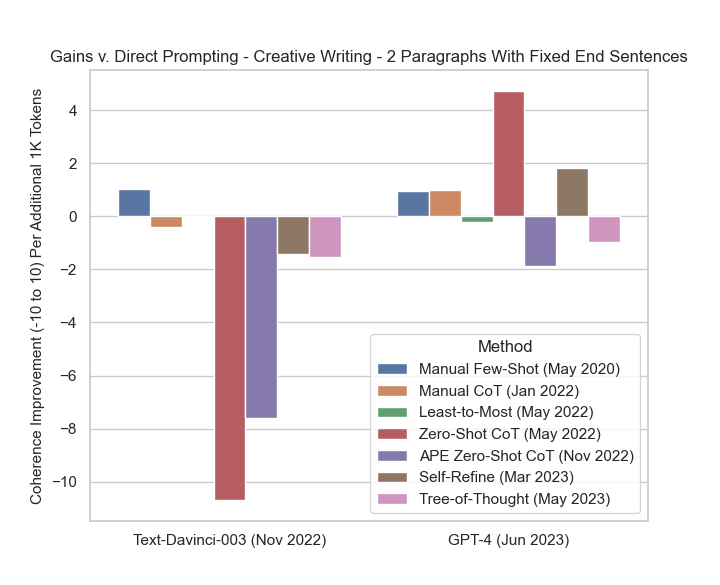
\includegraphics[width=0.95\hsize]{../Output/cw_change_in_accuracy_quality_per_change_in_conversation_length_sorted_by_technique_age_transformed.png}
  \end{subfigure}
  \hfill
\end{figure*}

%\twocolumn

For complexity, I report:

\begin{itemize}
  \item Number of reasoning steps - linebreaks, sentences (NLTK sentence tokenizer), strings "step i" and "1. ", "2. ", "3. ", etc. in the response \cite{fu_complexity-based_2023} \footnote{Sentences seem to be a better measure of complexity than just periods as were used in prior work (decimals, abbreviations, etc. present challenges though the problems can be mitigated somewhat with regex). Semicolons were also considered, but in experiments these did not appear unless models were specifically prompted towards including them. "step i" comes from \citealp{fu_complexity-based_2023}, but "1. ", "2. " etc. are novel metrics, to the best of my knowledge.}
  \item For Creative Writing: Sentence length (NLTK word and sentence tokenizers) in the response
  \item For Creative Writing: Flesch reading ease (implemented via the textstat Python package) in the response \cite{flesch_how_2016, aggarwal_textstat_nodate}
  \item Difference of the scores above in responses vs. prompts, additionally responses vs. provided answer for GSM8K
  \item For GSM8K: Human assessment of ease of review - on a scale of 1-10, how difficult is it to check the steps followed? GPT-4 can produce scalar scores on this, so I also collect its evaluations as an additional opinion (see Appendix Section \ref{sec:evaluating_ease_of_review}). Again, I report human scores, GPT-4 scores, the average of them, and Krippendorff's alpha.
\end{itemize}

%\begin{tabular}{llrrrrrrrr}
\toprule
model & task & direct_prompting & zero_shot_cot & ape_zero_shot_cot & tree_of_thought & self_refine & least_to_most & manual_few_shot & manual_cot \\
\midrule
gpt4 & cw & 63.776700 & 59.945100 & 60.737800 & 57.566700 & 62.369000 & 67.365100 & 67.843800 & 67.764000 \\
td3 & cw & 74.733700 & 72.385300 & 71.928000 & 66.679400 & 73.691800 & 75.954900 & 76.656700 & 74.101500 \\
gpt4 & gsm8k & NaN & NaN & NaN & NaN & NaN & NaN & NaN & NaN \\
td3 & gsm8k & NaN & NaN & NaN & NaN & NaN & NaN & NaN & NaN \\
\bottomrule
\end{tabular}


%\onecolumn

\begin{table*}
  \caption{Mean and Standard Deviation of Complexity Metrics}
  \centering
  \tiny
  \begin{tabular}{x{0.75cm}|x{1.5cm}|x{0.75cm}|x{0.75cm}|x{0.75cm}|x{0.75cm}|x{0.75cm}|x{0.75cm}|x{0.75cm}|x{0.75cm}|x{0.75cm}}
\toprule
\hline
Task & Metric & Model & Manual Few-Shot & Manual CoT & Least-to-Most & Zero-Shot CoT & APE Zero-Shot CoT & Self-Refine & Tree-of-Thought & Direct Prompting \\
\hline
\midrule
GSM8K & Number of Linebreaks & Text-Davinci-003 & 0.0* (0.0) & 0.0* (0.0) & 4.16* (3.41) & 3.25* (3.02) & 4.44* (5.6) & 1.16* (0.44) & 1.39* (0.87) & 0.16 (0.52) \\
\hline
 &  & GPT-4 & 0.0 (0.0) & 0.0 (0.0) & 0.0 (0.0) & 0.0 (0.0) & 0.0 (0.0) & 2.2* (0.97) & 5.11* (6.6) & 0.0 (0.0) \\
\hline
 & Number of Sentences & Text-Davinci-003 & 1.0* (0.0) & 4.96* (1.49) & 12.31* (9.37) & 4.66* (5.32) & 4.38* (9.05) & 2.25* (1.1) & 8.41* (11.4) & 1.49 (0.94) \\
\hline
 &  & GPT-4 & 1.0* (0.0) & 3.5* (2.37) & 8.59* (6.63) & 2.84* (2.58) & 3.15* (3.46) & 5.12* (5.32) & 8.03* (18.23) & 1.51 (0.33) \\
\hline
 & Number of Step 1, Step 2, etc. & Text-Davinci-003 & 0.0 (0.0) & 0.0 (0.0) & 0.0 (0.0) & 0.32* (1.05) & 0.56* (1.56) & 0.0 (0.0) & 2.0* (0.0) & 0.0 (0.0) \\
\hline
 &  & GPT-4 & 0.0 (0.0) & 0.0 (0.0) & 0.0 (0.0) & 0.0 (0.0) & 0.39* (1.31) & 0.0 (0.0) & 0.22 (1.75) & 0.0 (0.0) \\
\hline
 & Number of 1., 2., etc. & Text-Davinci-003 & 0.04* (0.04) & 2.54* (6.92) & 6.96* (9.37) & 1.84* (6.84) & 2.33* (10.49) & 0.5 (0.98) & 1.0 (0.0) & 0.72 (3.13) \\
\hline
 &  & GPT-4 & 0.04* (0.04) & 2.8* (13.72) & 6.95* (11.26) & 1.99 (13.2) & 1.95* (10.29) & 2.36* (19.28) & 3.5* (17.91) & 1.28 (8.89) \\
\hline
Creative Writing & Number of Linebreaks & Text-Davinci-003 & 1.07* (0.07) & 6.01* (0.25) & 7.03* (0.09) & 4.67* (6.08) & 4.37* (8.84) & 3.1* (2.37) & 11.29* (7.56) & 0.98 (0.06) \\
\hline
 &  & GPT-4 & 0.0 (0.0) & 0.0 (0.0) & 0.0 (0.0) & 0.0 (0.0) & 0.0 (0.0) & 1.56* (0.81) & 4.0* (0.0) & 0.0 (0.0) \\
\hline
 & Number of Sentences & Text-Davinci-003 & 10.08* (3.47) & 15.8* (2.97) & 17.82* (3.54) & 10.03* (5.69) & 10.12* (6.17) & 13.54* (28.8) & 31.37* (47.55) & 7.6 (1.78) \\
\hline
 &  & GPT-4 & 10.25* (3.56) & 11.93 (7.28) & 14.76* (6.0) & 15.92* (10.64) & 15.43* (15.18) & 15.97* (59.79) & 39.42* (38.21) & 11.32 (5.17) \\
\hline
 & Number of Step 1, Step 2, etc. & Text-Davinci-003 & 0.0 (0.0) & 0.0 (0.0) & 0.0 (0.0) & 1.71* (2.94) & 1.62* (3.19) & 0.0 (0.0) & 0.0 (0.0) & 0.0 (0.0) \\
\hline
 &  & GPT-4 & 0.0 (0.0) & 0.0 (0.0) & 0.0 (0.0) & 0.66* (2.97) & 0.9* (3.95) & 0.0 (0.0) & 0.0 (0.0) & 0.0 (0.0) \\
\hline
 & Number of 1., 2., etc. & Text-Davinci-003 & 0.01 (0.01) & 2.9* (0.21) & 2.99* (0.01) & 0.85* (1.4) & 0.51* (0.8) & 0.63* (0.62) & 2.84* (0.84) & 0.0 (0.0) \\
\hline
 &  & GPT-4 & 0.0 (0.0) & 0.94* (1.81) & 2.49* (0.49) & 3.58* (5.58) & 2.81* (7.21) & 0.8* (1.03) & 3.93* (2.19) & 0.0 (0.0) \\
\hline
 & Sentence Length & Text-Davinci-003 & 18.22 (6.6) & 16.26* (2.72) & 15.06* (2.13) & 17.53* (12.88) & 18.26 (15.96) & 16.43* (5.03) & 21.21* (10.41) & 18.36 (7.11) \\
\hline
 &  & GPT-4 & 21.3* (7.93) & 21.16* (9.85) & 20.95* (7.56) & 22.05 (17.5) & 23.32 (30.69) & 21.36* (5.53) & 24.87* (9.58) & 22.61 (8.86) \\
\hline
 & Flesch Reading Ease Score & Text-Davinci-003 & 76.66* (57.45) & 74.1 (38.72) & 75.95 (32.47) & 72.39* (72.85) & 71.93* (78.95) & 73.69 (61.79) & 66.68* (66.79) & 74.73 (67.91) \\
\hline
 &  & GPT-4 & 67.84* (55.25) & 67.76* (51.02) & 67.37* (35.66) & 59.95* (50.18) & 60.74* (44.73) & 62.37 (51.28) & 57.57* (43.82) & 63.78 (51.29) \\
\hline
\bottomrule
\end{tabular}
  
  \label{tab:avg_complexity_metrics_pivot}
  \newline \newline \footnotesize Stars indicate a significant difference from the direct prompting baseline from paired t-tests at the 95\% level.
\end{table*}

\begin{table*}
  \caption{Differences of Complexity Metrics}
  \centering
  \tiny
  \begin{tabular}{x{0.75cm}|x{1.5cm}|x{0.75cm}|x{0.75cm}|x{0.75cm}|x{0.75cm}|x{0.75cm}|x{0.75cm}|x{0.75cm}|x{0.75cm}|x{0.75cm}}
\toprule
\hline
Task & Metric & Model & Manual Few-Shot & Manual CoT & Least-to-Most & Zero-Shot CoT & APE Zero-Shot CoT & Self-Refine & Tree-of-Thought & Direct Prompting \\
\hline
\midrule
GSM8K & Difference in Number of Linebreaks (Responses - Prompts) & Text-Davinci-003 & 16.0 & 16.0 & 1.84 & -1.25 & -2.44 & 1.84 & 4.0 & 0.84 \\
\hline
 &  & GPT-4 & 16.0 & 14.83 & -0.64 & -1.83 & -2.64 & 0.03 & -6.15 & -0.34 \\
\hline
 & Difference in Number of Sentences (Responses - Prompts) & Text-Davinci-003 & 28.36 & 57.4 & 4.05 & -0.3 & -0.02 & 5.11 & -2.18 & 2.87 \\
\hline
 &  & GPT-4 & 19.36 & 42.86 & 2.77 & 0.52 & 0.21 & 1.44 & 15.75 & 1.85 \\
\hline
 & Difference in Number of Step 1, Step 2, etc. (Responses - Prompts) & Text-Davinci-003 & 0.0 & 0.0 & 0.0 & -0.32 & -0.56 & 0.0 & -2.0 & 0.0 \\
\hline
 &  & GPT-4 & 0.0 & 0.0 & 0.0 & 0.0 & -0.39 & 0.0 & 1.78 & 0.0 \\
\hline
 & Difference in Number of 1., 2., etc. (Responses - Prompts) & Text-Davinci-003 & 6.34 & 17.84 & -2.58 & -1.46 & -1.95 & -0.12 & 1.83 & -0.34 \\
\hline
 &  & GPT-4 & 6.34 & 17.58 & -2.57 & -1.61 & -1.57 & -1.98 & -2.12 & -0.9 \\
\hline
 & Difference in Number of Linebreaks (Responses - Provided Answer) & Text-Davinci-003 & 3.42 & 3.42 & -0.74 & 0.17 & -1.02 & 2.26 & 2.03 & 3.26 \\
\hline
 &  & GPT-4 & 3.42 & 2.25 & -2.22 & -0.41 & -1.22 & -1.95 & -8.84 & 2.08 \\
\hline
 & Difference in Number of Sentences (Responses - Provided Answer) & Text-Davinci-003 & 1.68 & -2.28 & -9.63 & -1.98 & -1.7 & 0.43 & -5.73 & 1.19 \\
\hline
 &  & GPT-4 & 1.68 & -0.82 & -5.91 & -0.16 & -0.47 & -2.44 & -5.35 & 1.17 \\
\hline
 & Difference in Number of Step 1, Step 2, etc. (Responses - Provided Answer) & Text-Davinci-003 & 0.0 & 0.0 & 0.0 & -0.32 & -0.56 & 0.0 & -2.0 & 0.0 \\
\hline
 &  & GPT-4 & 0.0 & 0.0 & 0.0 & 0.0 & -0.39 & 0.0 & -0.22 & 0.0 \\
\hline
 & Difference in Number of 1., 2., etc. (Responses - Provided Answer) & Text-Davinci-003 & 1.24 & -1.26 & -5.68 & -0.56 & -1.05 & 0.78 & 0.28 & 0.56 \\
\hline
 &  & GPT-4 & 1.24 & -1.52 & -5.67 & -0.71 & -0.67 & -1.08 & -2.22 & 0.0 \\
\hline
Creative Writing & Difference in Number of Linebreaks (Responses - Prompts) & Text-Davinci-003 & 7.93 & 12.99 & 11.97 & -4.67 & -4.37 & 1.52 & -6.29 & -0.98 \\
\hline
 &  & GPT-4 & 6.99 & 15.31 & 11.5 & -10.93 & -10.77 & -0.25 & -13.54 & -2.08 \\
\hline
 & Difference in Number of Sentences (Responses - Prompts) & Text-Davinci-003 & 24.91 & 31.19 & 33.17 & -4.05 & -4.14 & -4.34 & -18.38 & -2.61 \\
\hline
 &  & GPT-4 & 17.74 & 23.06 & 22.23 & -9.94 & -9.45 & -9.7 & -27.43 & -6.33 \\
\hline
 & Difference in Number of Step 1, Step 2, etc. (Responses - Prompts) & Text-Davinci-003 & 0.0 & 0.0 & 0.0 & -1.71 & -1.62 & 0.0 & 0.0 & 0.0 \\
\hline
 &  & GPT-4 & 0.0 & 0.0 & 0.0 & -0.66 & -0.9 & 0.0 & 0.0 & 0.0 \\
\hline
 & Difference in Number of 1., 2., etc. (Responses - Prompts) & Text-Davinci-003 & 5.99 & 9.1 & 9.01 & 1.15 & 1.49 & 2.77 & -0.84 & 2.0 \\
\hline
 &  & GPT-4 & 6.0 & 11.06 & 9.51 & -1.58 & -0.81 & 2.48 & -1.93 & 2.0 \\
\hline
 & Difference in Sentence Length (Responses - Prompts) & Text-Davinci-003 & -4.54 & -2.82 & -1.64 & -7.15 & -6.19 & -2.96 & -6.38 & -7.77 \\
\hline
 &  & GPT-4 & -3.37 & -2.62 & -2.14 & -9.92 & -9.36 & -0.46 & -6.01 & -9.86 \\
\hline
 & Difference in Flesch Reading Ease Score (Responses - Prompts) & Text-Davinci-003 & -1.66 & 0.14 & -2.07 & 7.05 & 5.48 & 3.16 & 11.72 & 7.51 \\
\hline
 &  & GPT-4 & 7.29 & 5.56 & 6.87 & 17.69 & 14.96 & 8.64 & 15.83 & 15.42 \\
\hline
\bottomrule
\end{tabular}
  
  \label{tab:avg_complexity_diff_metrics_pivot}
\end{table*}

%\clearpage

%\twocolumn

General Discussion:

As is the case for chain-of-thought prompting in the setting of \citealp{fu_complexity-based_2023}, are any gains in performance coming from reasoning steps as opposed to length (of the prompt or overall interaction, in tokens)? This question is central to our understanding of if and how prompt engineering works. Relationships may be complex. For language understanding tasks, prompt length has been found to improve model performance, with optimality achieved somewhere in the range of 20-100 tokens \cite{lester_power_2021}. Evidence shows that in longer conversations models may get distracted, go off on tangents, or get stuck in a loop repeating themselves (to the extent some platforms have imposed length limitations) \cite{shi_large_2023, mann_microsoft_nodate}. A conversation level logistic regression (with quadratic terms to model non-linearity) controlling for length and complexity can provide insight. Standard errors should be clustered by the identity of the question and method.

Does increased length or complexity limit creativity and randomness? Investigating regression results on the creative writing task in particular might be helpful - coherence requires creativity. Variance/standard deviations in scores may also offer insights.

Does increased prompted complexity lead to worse performance on simple questions? For GSM8K, we can use the complexity of provided answers to get a measure of how simple the question is, and add this as an interaction in the regression. The results from this paper can help resolve debate in the chain-of-thought literature. \cite{fu_complexity-based_2023, shum_automatic_2023}

To what extent does prompting require specialized skills and time investment? Appendix Section \ref{sec:difficulty} offers some observations on the difficulty of implementing each method covered in this paper. Length and metrics for the output and ease of review scores in particular may provide insight into checking results - the other part of the prompting process.

%\onecolumn

\begin{table*}
  \caption{Regression Results}
  \centering
  \tiny
  \begin{tabular}{x{1.5cm}|x{0.75cm}|x{0.75cm}|x{0.75cm}|x{0.75cm}|x{0.75cm}|x{0.75cm}}
\toprule
\hline
Model & Conversation Length (Thousands of Tokens) & Conversation Length (Thousands of Tokens) Squared & Number of Steps/Ideas & Number of Steps/Ideas Squared & Flesch Reading Ease & Flesch Reading Ease Squared \\
\hline
\midrule
GSM8K Correct, Logit & 0.277 (0.143) & -0.498* (0.127) & 0.029* (0.007) & -0.002* (0.0) &  &  \\
\hline
GSM8K Correct, Linear & 0.282* (0.114) & -0.418* (0.091) & 0.043* (0.006) & -0.002* (0.0) &  &  \\
\hline
Creative Writing Cosine Similarity & 0.212* (0.045) & -0.119* (0.03) & 0.01* (0.004) & -0.0 (0.001) & -0.011* (0.004) & 0.0* (0.0) \\
\hline
Creative Writing Compliance, Logit & -0.557* (0.161) & 0.23* (0.11) & -0.025 (0.018) & 0.005 (0.003) & 0.041* (0.017) & -0.0* (0.0) \\
\hline
Creative Writing Compliance, Linear & -0.531* (0.158) & 0.226* (0.107) & -0.033* (0.016) & 0.006* (0.003) & 0.045* (0.016) & -0.0* (0.0) \\
\hline
\bottomrule
\end{tabular}
  
  \label{tab:regressions}
  \newline \newline \footnotesize For logit regressions, the average of marginal effects are reported. Standard errors in parentheses. For linear models, standard errors are clustered by task question by method. Stars indicate significance at the 95\% level.
\end{table*}

\begin{table*}
  \caption{Regressions with GSM8K Provided Answer Length Interaction}
  \centering
  \tiny
  \begin{tabular}{x{1.5cm}|x{0.75cm}|x{0.75cm}|x{0.75cm}|x{0.75cm}|x{0.75cm}|x{0.75cm}|x{0.75cm}|x{0.75cm}|x{0.75cm}}
\toprule
\hline
Model & Length * Provided Length & Number of Steps/Ideas * Provided Length & Length Squared * Provided Length & Number of Steps/Ideas Squared * Provided Length & Conversation Length & Number of Steps/Ideas & Conversation Length Squared & Number of Steps/Ideas Squared & Provided Length \\
\hline
\midrule
GSM8K Correct, Logit & -5.091 (3.57) & 0.087 (0.168) & 2.908 (3.266) & 0.003 (0.011) & 0.739 (0.413) & 0.027 (0.019) & -0.699 (0.433) & -0.002 (0.001) & -1.216 (0.982) \\
\hline
GSM8K Correct, Linear & -5.303 (2.85) & 0.005 (0.176) & 1.786 (2.19) & -0.001 (0.012) & 0.71* (0.346) & 0.041* (0.02) & -0.513 (0.327) & -0.002 (0.002) & -6.541 (124.292) \\
\hline
\bottomrule
\end{tabular}
  
  \label{tab:regressions_provided_interaction}
  \newline \newline \footnotesize For logit regressions, the average of marginal effects are reported. Standard errors in parentheses. For linear models, standard errors are clustered by task question by method. Stars indicate significance at the 95\% level.
\end{table*}

\begin{table*}
  \caption{Regressions with Model Interaction}
  \centering
  \tiny
  \begin{tabular}{x{1.5cm}|x{0.75cm}|x{0.75cm}|x{0.75cm}|x{0.75cm}|x{0.75cm}|x{0.75cm}|x{0.75cm}|x{0.75cm}|x{0.75cm}|x{0.75cm}|x{0.75cm}|x{0.75cm}|x{0.75cm}|x{0.75cm}}
\toprule
\hline
Model & Conversation Length * Model = TD3 & Number of Steps/Ideas * Model = TD3 & Conversation Length Squared * Model = TD3 & Number of Steps/Ideas Squared * Model = TD3 & Flesch Reading Ease * Model = TD3 & Flesch Reading Ease Squared * Model = TD3 & Conversation Length & Number of Steps/Ideas & Conversation Length Squared & Number of Steps/Ideas Squared & Flesch Reading Ease & Flesch Reading Ease Squared & Model = TD3 \\
\hline
\midrule
GSM8K Correct, Logit & -0.403 (0.401) & 0.003 (0.014) & 1.081* (0.439) & 0.0 (0.001) &  &  & -0.196 (0.236) & 0.031* (0.01) & -0.229 (0.181) & -0.002* (0.001) &  &  & -0.453* (0.076) \\
\hline
GSM8K Correct, Linear & -0.449 (0.365) & 0.009 (0.012) & 1.092* (0.439) & -0.0 (0.001) &  &  & -0.076 (0.146) & 0.043* (0.007) & -0.228* (0.104) & -0.002* (0.0) &  &  & -0.469* (0.059) \\
\hline
Creative Writing Cosine Similarity & 0.277* (0.123) & -0.02 (0.012) & -0.108 (0.095) & 0.004 (0.003) & -0.003 (0.012) & 0.0 (0.0) & -0.053 (0.064) & 0.014* (0.005) & 0.018 (0.039) & -0.001 (0.001) & -0.013* (0.006) & 0.0* (0.0) & 0.025 (0.438) \\
\hline
Creative Writing Compliance, Logit & -0.166 (0.467) & -0.023 (0.041) & -0.071 (0.365) & 0.002 (0.009) & -0.0 (0.047) & 0.0 (0.0) & -0.118 (0.256) & -0.009 (0.022) & 0.004 (0.153) & 0.003 (0.004) & 0.056 (0.029) & -0.0 (0.0) & -0.231 (1.627) \\
\hline
Creative Writing Compliance, Linear & -0.276 (0.424) & 0.003 (0.042) & 0.01 (0.321) & -0.005 (0.009) & -0.003 (0.046) & 0.0 (0.0) & -0.058 (0.248) & -0.023 (0.02) & -0.012 (0.149) & 0.006* (0.003) & 0.053* (0.026) & -0.0 (0.0) & 0.35 (1.628) \\
\hline
\bottomrule
\end{tabular}
  
  \label{tab:regressions_model_interaction}
  \newline \newline \footnotesize For logit regressions, the average of marginal effects are reported. Standard errors in parentheses. For linear models, standard errors are clustered by task question by method. Stars indicate significance at the 95\% level.
\end{table*}

%\twocolumn

\section*{Conclusion}

Overarching conclusions about the practicality of prompt engineering and the tradeoffs between costs and benefits of specific techniques.

\section*{Limitations}

It was difficult to select prompt engineering methods to try for this paper, and there is potential for my choice of methods to be somewhat biased. I mostly picked methods based my perception of their popularity and ease of implementation. If anything, this may lead to an underestimation of net costs if easy-to-implement and high quality methods are likely to be popular. 

Though I believe that the evaluation tasks I selected represent a wide range of areas in which LLMs may be useful - logical reasoning/problem solving, and creativity - they are not comprehensive, and different adaptations of prompting methods to different tasks may lead to different results.

Just as my evaluation comes at a time with significantly more capable LLMs relative to those available when much work began on prompting, I expect the underlying calculus concerning prompting to continue to change in the future. However, I again only expect relative costs of complex engineering to increase as models get better.

Another potential problem is the extent that prompting techniques have been absorbed into default LLM behavior, likely through reinforcement learning. GPT-4 in particular does seem to automatically implement chain-of-thought methods when presented with a sufficiently complex problem. In this environment, this paper become less of an evaluation of prompting techniques themselves, but more of an evaluation of their intentional and manual implementation.

Due to the inherently unstable nature of LLM performance even in a fixed environment, and their broad and critical implications for society, there is great value even in testing models with exactly the same questions and prompts repeatedly. The statistical robustness of results from this paper and others should be tested repeatedly in future research.

\section*{Acknowledgements}
This document was created from a template made by Jordan Boyd-Graber, Naoaki Okazaki, and Anna Rogers.

\bibliography{custom}
\bibliographystyle{acl_natbib}

\clearpage
\newpage

\onecolumn
\setlength{\parindent}{0cm}
\setlength\parskip{1em plus 0.1em minus 0.2em}
\appendix

\section{The Popularity of Some Prompting Methods}
\label{sec:popularity}

Table \ref{tab:method_pop} displays the popularity (in terms of Semantic Scholar citations) of some of the most popular generalizable prompt engineering methods based on the lists at \url{https://www.promptingguide.ai/papers#approaches} and \url{https://en.wikipedia.org/wiki/Prompt_engineering#Text-to-text} as of October 22, 2023. Please contact the author for a full list of the 162 papers considered.

Another good resource for prompt engineering methods and evaluations is the paperswithcode website: \url{https://paperswithcode.com/task/prompt-engineering}. I did not make use of this page, however, as it seemed to be missing many prominent approaches, contains text-to-vision methods, and focuses on GitHub implementations (which are often low integer numbers difficult to compare) and currently trending social media items.

\begin{landscape}

  \begin{centering}

    \begin{table}[h]
      \caption{Popularity of Selected Prompt Engineering Methods}
      \small
      \begin{tabular}{llc}
\toprule
Paper Title & Prompt Engineering Method & Citations Per Day Since Release \\
\midrule
Language Models are Few-Shot Learners & Few-Shot Learning & 13.23 \\
Chain of Thought Prompting Elicits Reasoning in Large Language Models & Chain-of-Thought Prompting & 3.33 \\
Large Language Models are Zero-Shot Reasoners & Zero-Shot Chain-of-Thought & 1.71 \\
Tree of Thoughts: Deliberate Problem Solving with Large Language Models & Tree-of-Thought & 1.43 \\
Self-Refine: Iterative Refinement with Self-Feedback & Self-Refine & 0.97 \\
ReAct: Synergizing Reasoning and Acting in Language Models & ReAct & 0.87 \\
Least-to-most prompting enables complex reasoning in large language models & Least-to-Most Prompting & 0.71 \\
PAL: Program-aided Language Models & Program Aided Language Models & 0.58 \\
Large Language Models Are Human-Level Prompt Engineers & Automatic Prompt Engineer & 0.55 \\
How Can We Know What Language Models Know? & Prompt Mining, Prompt Paraphrasing & 0.54 \\
Automatic Chain of Thought Prompting in Large Language Models & Automatic Chain of Thought Prompting & 0.53 \\
Show Your Work: Scratchpads for Intermediate Computation with Language Models & Scratchpads & 0.46 \\
Multimodal Chain-of-Thought Reasoning in Language Models & Multimodal CoT & 0.35 \\
Prompt Programming for Large Language Models: Beyond the Few-Shot Paradigm & Metaprompt & 0.32 \\
CAMEL: Communicative Agents for "Mind" Exploration of Large Scale Language Model Society & Role-Playing & 0.31 \\
Chain-of-Verification Reduces Hallucination in Large Language Models & Chain-of-Verification & 0.31 \\
Complexity-Based Prompting for Multi-Step Reasoning & Complexity-Based Prompting & 0.3 \\
Decomposed Prompting: A Modular Approach for Solving Complex Tasks & Decomposed Prompting & 0.27 \\
Plan-and-Solve Prompting: Improving Zero-Shot Chain-of-Thought Reasoning by Large Language Models & Plan-and-Solve Prompting & 0.27 \\
Large Language Models Can Be Easily Distracted by Irrelevant Context & Instruction to Ignore Irrelevant Information & 0.26 \\
Connecting Large Language Models with Evolutionary Algorithms Yields Powerful Prompt Optimizers & EvoPrompt & 0.21 \\
AI Chains: Transparent and Controllable Human-AI Interaction by Chaining Large Language Model Prompts & Chaining & 0.2 \\
Prompting GPT-3 To Be Reliable & Prompting for Reliability & 0.19 \\
Demonstrate-Search-Predict: Composing retrieval and language models for knowledge-intensive NLP & Demonstrate-Search-Predict & 0.19 \\
ART: Automatic multi-step reasoning and tool-use for large language models & Automatic Reasoning and Tool-Use & 0.18 \\
Promptagator: Few-Shot Dense Retrieval From 8 Examples & Few-Shot Dense Retrieval & 0.17 \\
Maieutic Prompting: Logically Consistent Reasoning with Recursive Explanations & Maieutic Prompting & 0.17 \\
Reframing Instructional Prompts to GPTk's Language & Reframing & 0.16 \\
Generated Knowledge Prompting for Commonsense Reasoning & Generated Knowledge Prompting & 0.15 \\
Teaching Algorithmic Reasoning via In-context Learning & Algorithmic Prompting & 0.15 \\
Hard Prompts Made Easy: Gradient-Based Discrete Optimization for Prompt Tuning and Discovery & Gradient-Based Prompt Optimization & 0.15 \\
\bottomrule
\end{tabular}

      \label{tab:method_pop}
    \end{table}

  \end{centering}

\end{landscape}

\clearpage
\newpage

\section{Average Inter-Paragraph Cosine Similarity Examples}
\label{sec:avg_inter_pragraph_cosine_sim_ex}

\subsection*{Inter-Paragraph Cosine Simlarity: 0.01} %0.0096024028634174

Learning to do a handstand is a fun activity for people of all ages. It takes practice to master, but once you get the hang of it, you'll learn to balance your body in an upside-down position. It isn't difficult to do a handstand if you just stand on your hands.

John, a space explorer, felt excited when he first stepped on the moon. It was a unique experience that he thought he would never forget. To his surprise, a smell of seared steak followed him up the mountain of dust. It caught him off guard that space smelled of seared steak.

\subsection*{Inter-Paragraph Cosine Simlarity: 0.25} %0.250084849757387

The explorers were fascinated in equal parts fear and curiosity as they surveyed the unfamiliar terrain of this new planet. A unique alien species of flora, turning the water around it a shocking ochre, was the planet's highlight, causing a stark contrast to the otherwise jade green surroundings. Trembling hands reached out towards the phenomenon, a capsule took a sample, and rigorous testing was conducted. Initial concerns turned to relieved laughter when the tests ran positive. Just because the water is red doesn't mean you can't drink it.

The day ended, and the crew retreated to the layered confines of their habitat module. The walls were littered with mission updates and data charts, each element portraying the organized chaos of their voyage. In the space assigned for leisure, a small wooden table, reminiscent of Earth, was cluttered with mugs and a single book. Earlier discussions and laughter started to die out, replaced by the hum of computers and machines as each of them turned to their individual activities. Amidst this controlled mayhem, the book lay untouched, a visual metaphor of their longing for home and comfort. The book is in front of the table.

\subsection*{Inter-Paragraph Cosine Simlarity: 0.5} %0.504750327816827

The sun beat down heavily on the sandy beach, and the smell of the salty ocean air mixed with the humidity. Suddenly, thick rain clouds appeared overhead and the looking sky filled with a dark shade of grey. The rain came in quickly, quickly, washing the thick sand into the ocean with a powerful force. Just as the storm intensified, she peered out over the horizon and saw something unexpected--a few crocodiles were launched into the water by the mass of the flooding rain. The sudden rainstorm washed crocodiles into the ocean.

She watched in appreciation as the creatures navigated the swells of the ocean, slipping out and in of view as the waves rose and fell. There was something meditative about it--the way the rain mixed with the sky--and she was mesmerized. Her gaze eventually fell on the man a few feet from her, watching the same scene unfold. She wondered what his eyes were saying beneath his mirrored sunglasses.

\subsection*{Inter-Paragraph Cosine Simlarity: 0.75} %0.746425791603845

Elsa had been feeling lost since she graduated college. She hadn't found her passion in life yet and was looking for a way to feel purposeful and fulfilled. She decided to spend some of her savings on a road trip. She wanted to reclaim the feeling of being free that she had when she was a child, and the open road seemed like the way to do that. So, she grabbed her map and a duffle bag, and hit the highway. Her hair was windswept as she rode in the black convertible.

It took her to a small village in the mountains far from the city. She had days filled with new people, food, and experiences. She even took the time to learn some new skills and hobbies. She traveled because it cost the same as therapy and was a lot more enjoyable. As the miles rolled by, she came to understand that by living intentionally and being courageous, one can find a second chance at life.

\begin{figure}[h]
  \caption{Histogram - Average Inter-Paragraph Cosine Similarity}
  \centering
  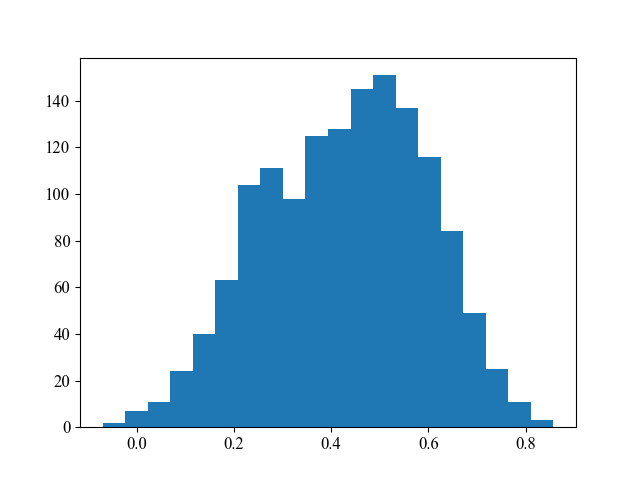
\includegraphics[width=\textwidth]{../Output/avg_inter_paragraph_cosine_sim_hist.png}
  \label{fig:avg_inter_paragraph_cosine_sim_hist}
\end{figure}

\clearpage
\newpage

\section{Notes on Ease of Implementation}
\label{sec:difficulty}

Here are my rough evaluations of the difficulty of implementing each method selected for this paper. Ratings are on a scale from 1-6, with 1 being the easiest.

\subsubsection*{Zero-Shot Methods}

Rating: 1. These methods append a common string to the prompt that is extremely similar for all tasks.

\subsubsection*{Manual Few-Shot}

Rating: 2. A few examples of questions and solutions must be provided, but these are usually relatively easy to find.

\subsubsection*{Few-Shot Least-to-Most}

Rating: 3. A little more detail must be added to chain of thought solutions to demonstrate the structure behind splitting a problem into subproblems.

\subsubsection*{Manual Chain-of-Thought}

Rating: 4. Worked questions and solutions must be provided, but these are usually not very difficult to find - a good share of provided solutions also include explanations.

\subsubsection*{Self-Refine}

Rating: 5. Many of the same considerations as the Tree-of-Thought method apply. However, the feedback-refinement loop is somewhat simpler than a tree structure.

\subsubsection*{Tree-of-Thought}

Rating: 6. A specific search tree structure and a method for traversing it must be constructed. This can vary a lot depending on the task - considerations are breadth-first versus depth-first, how many nodes/possibilities to consider at each step, etc. It is also necessary to consider how to structure a feedback loop where the LLM takes into account its previous responses. Any instructions must be simple enough for the LLM to follow.

\clearpage
\newpage

\section{Notes on Ease of Review}
\label{sec:ease_of_review}

Here are my rough evaluations of the difficulty of reviewing the output of each method selected for this paper. Ratings are on a scale from 1-6, with 1 being the easiest.

\subsubsection*{Manual Few-Shot, Manual Chain-of-Thought}

Rating: 1. The prompt design and examples provided intentionally make it extremely easy to check the final answer - output is consistently formatted.

\subsubsection*{Direct Prompting}

Rating: 2. The LLM responses are usually direct and the lack of extra instructions makes the output simple. 

\subsubsection*{Zero-Shot Chain-of-Thought, APE Improved Zero-Shot Chain-of-Thought}

Rating: 3. The steps the model takes for each individual problem and their formatting can be inconsistent. On the other hand, the steps are usually clearly spelled out, and the final answer or passage is usually fairly clear.

\subsubsection*{Self-Refine}

Rating: 4. Self-Refine is an iterative process across several pieces of dialogue, though they do follow a simple structure.

\subsubsection*{Least-to-Most Prompting}

Rating: 5. The planning and execution sets of steps of Least-to-Most Prompting can be hard to untangle and piece back together.

\subsubsection*{Tree-of-Thought}

Rating: 6. Specific steps are split up across many pieces of dialogue and many potential tree branches, potentially with backtracking, and it is difficult to reconstruct the entire chain of logic and actions.

\clearpage
\newpage

\section{Prompts Used}
\label{sec:prompts}

Below I have listed question and prompt examples for each task and method.

\subsection{GSM8K}

The sample problem below is the first one in the GSM8K test dataset. \cite{cobbe_training_2021}

<Question> "Janet's ducks lay 16 eggs per day. She eats three for breakfast every morning and bakes muffins for her friends every day with four. She sells the remainder at the farmers' market daily for \$2 per fresh duck egg. How much in dollars does she make every day at the farmers' market?"

All prompt examples for few-shot methods come from the training dataset.

\subsubsection*{Zero-Shot Control Baseline/Direct Prompting}

Q: <Question>

A:

\subsubsection*{Zero-Shot Chain-of-Thought}

Q: <Question>

A: Let's think step by step.

\subsubsection*{APE Improved Zero-Shot Chain-of-Thought}

Q: <Question>

A: Let's work this out in a step by step way to be sure we have the right answer.

\subsubsection*{Tree-of-Thought}

Q: <Question>

Task: Generate 3 different possible one-step calculations to serve as step 1 in solving the problem. Only work on step 1. Put each calculation on a new line. Do not number them.

<Response>

Task: State the calculation above that is most likely to contribute to solving the problem. If it fully solves the original problem, also output STOP and the solution to the problem. If none of the calculations are correct, output ERROR and generate three new ones.

<Response>

Task: Generate 3 different possible one-step calculations to serve as the next step in solving the problem. Only work on the next step. Put each calculation on a new line. Do not number them.

<Response>

\subsubsection*{Self-Refine}

Q: <Question>

A: <Response>

Task: Please check the answer above. If there is an error, state what the error is, but don't fix it. If there are no errors, output STOP.

Feedback: <Feedback>

Task: Redo the entire problem based on the most recent feedback.

A: <Response>

\subsubsection*{Least-to-most Prompting (1-shot; taken from p.58 of \citealp{zhou_least--most_2023})}

Q: Elsa has 5 apples. Anna has 2 more apples than Elsa. How many apples do they have together?

A: Let's break down this problem: 1. How many apples does Anna have? 2. How many apples do Elsa and Anna have together?

1. Anna has 2 more apples than Elsa. So Anna has 2 + 5 = 7 apples.

2. Elsa and Anna have 5 + 7 = 12 apples together.

Q: <Question>

A: Let's break down this problem:

\subsubsection*{Manual Few-Shot (randomly drawn questions and final answers from the training set - following the methodology on p.10 \citealp{brown_language_2020}. 8 examples were chosen, so as to enable comparison with the Chain-of-Thought exemplars below, and in light of evidence that this is around the optimal number of exemplars \cite{min_rethinking_2022}. Explanations were removed from the answers.)}

Q: For every 12 cans you recycle, you receive \$0.50, and for every 5 kilograms of newspapers, you receive \$1.50. If your family collected 144 cans and 20 kilograms of newspapers, how much money would you receive?

A: 12

Q: Betty picked 16 strawberries. Matthew picked 20 more strawberries than Betty and twice as many as Natalie. They used their strawberries to make jam. One jar of jam used 7 strawberries and they sold each jar at \$4. How much money were they able to make from the strawberries they picked?

A: 40

Q: Jack has a stack of books that is 12 inches thick. He knows from experience that 80 pages is one inch thick. If he has 6 books, how many pages is each one on average?

A: 160

Q: James dumps his whole collection of 500 Legos on the floor and starts building a castle out of them.  He uses half the pieces before finishing and is told to put the rest away.  He puts all of the leftover pieces back in the box they came from, except for 5 missing pieces that he can't find.  How many Legos are in the box at the end?

A: 245

Q: Ines had \$20 in her purse. She bought 3 pounds of peaches, which are \$2 per pound at the local farmers' market. How much did she have left?

A: 14

Q: Aaron pays his actuary membership fees each year. The membership fee increases yearly by \$10. If he pays \$80 in the first year, how much does his membership cost, in dollars, in the sixth year?

A: 130

Q: Joseph invested \$1000 into a hedge fund. The fund promised a yearly interest rate of 10\%. If he deposited an additional \$100 every month into the account to add to his initial investment of \$1000, how much money will he have in the fund after two years?

A: 3982

Q: The price of buying a wooden toy at the new Craftee And Best store is \$20, and the cost of buying a hat is \$10. If Kendra went to the shop with a \$100 bill and bought two wooden toys and three hats, calculate the change she received.

A: 30

Q: <Question>

A:

\subsubsection*{Manual Chain-of-Thought (taken from p.35 of \citealp{wei_chain--thought_nodate})}

Q: There are 15 trees in the grove. Grove workers will plant trees in the grove today. After they are done, there will be 21 trees. How many trees did the grove workers plant today?

A: There are 15 trees originally. Then there were 21 trees after some more were planted. So there must have been 21 - 15 = 6. The answer is 6.

Q: If there are 3 cars in the parking lot and 2 more cars arrive, how many cars are in the parking lot?

A: There are originally 3 cars. 2 more cars arrive. 3 + 2 = 5. The answer is 5.

Q: Leah had 32 chocolates and her sister had 42. If they ate 35, how many pieces do they have left in total?

A: Originally, Leah had 32 chocolates. Her sister had 42. So in total they had 32 + 42 = 74. After eating 35, they had 74 - 35 = 39. The answer is 39.

Q: Jason had 20 lollipops. He gave Denny some lollipops. Now Jason has 12 lollipops. How many lollipops did Jason give to Denny?

A: Jason started with 20 lollipops. Then he had 12 after giving some to Denny. So he gave Denny 20 - 12 = 8. The answer is 8.

Q: Shawn has five toys. For Christmas, he got two toys each from his mom and dad. How many toys does he have now?

A: Shawn started with 5 toys. If he got 2 toys each from his mom and dad, then that is 4 more toys. 5 + 4 = 9. The answer is 9.

Q: There were nine computers in the server room. Five more computers were installed each day, from monday to thursday. How many computers are now in the server room?

A: There were originally 9 computers. For each of 4 days, 5 more computers were added. So 5 * 4 = 20 computers were added. 9 + 20 is 29. The answer is 29.

Q: Michael had 58 golf balls. On tuesday, he lost 23 golf balls. On wednesday, he lost 2 more. How many golf balls did he have at the end of wednesday?

A: Michael started with 58 golf balls. After losing 23 on tuesday, he had 58 - 23 = 35. After losing 2 more, he had 35 - 2 = 33 golf balls. The answer is 33.

Q: Olivia has \$23. She bought five bagels for \$3 each. How much money does she have left?

A: Olivia had 23 dollars. 5 bagels for 3 dollars each will be 5 x 3 = 15 dollars. So she has 23 - 15 dollars left. 23 - 15 is 8. The answer is 8.

Q: <Question>

A:

\subsection{Creative Writing}

The sample task below is the first one in the Creative Writing dataset. \cite{yao_tree_2023}

<Task> Write a coherent passage of 2 short paragraphs. The end sentence of each paragraph must be: 1. It isn't difficult to do a handstand if you just stand on your hands. 2. It caught him off guard that space smelled of seared steak. \footnote{Some preliminary experiments replacing the first sentence with "Write a coherent passage of 2 short paragraphs that flow together.", which seemed to improve zero-shot performance. This seems to nudge the model away from writing two unrelated paragraphs ending in the selected sentences - a flaw it often notices when asked for feedback on its own passages. However, I decided not to adopt this modification to stay in line with the original task.}

No training data was provided, so I used random sentences courtesy of \url{https://www.thewordfinder.com/random-sentence-generator/} and my own answers in the construction of few-shot examples.

\subsubsection*{Zero-Shot Control Baseline/Direct Prompting}

<Task>

\subsubsection*{Zero-Shot Chain-of-Thought}

<Task>. Plan step-by-step before writing the passage.

\subsubsection*{APE Improved Zero-Shot Chain-of-Thought}

<Task>. Plan step-by-step before writing the passage to be sure we have a correct and coherent answer.

\subsubsection*{Tree-of-Thought}

<Modified Task. Example: Goal: A coherent passage of 2 short paragraphs. The end sentence of each paragraph, respectively, must be: 1. It isn't difficult to do a handstand if you just stand on your hands. 2. It caught him off guard that space smelled of seared steak.>

Your Task: Generate 3 one-sentence plans for potential passages. Only generate one-sentence plans - do not write the passage.

<Response>

Your Task: Select the most coherent plan that follows the rules of the task. Only state the plan - do not write the passage.

<Response>

Your Task: Write 3 drafts of the 2-paragraph passage based on this plan.

<Response>

Your Task: Select the most coherent draft that follows the rules of the task and write it out.

<Response>

Your Task: If the draft is correct and coherent to the extent you would award a 10 on a scale of 1 to 10, output STOP. If it is not, write out a different one-sentence plan for a potential passage from among those considered and output PLAN.

<Response>

\subsubsection*{Self-Refine}

Task: <Task>

Response: <Response>

Your Task: Provide feedback on the correctness and coherence of the response and a rating on a scale of 1-10. If it is already coherent and correct to the extent you would award a 10, output 10 and the word STOP.

Feedback: <Feedback>

Your Task: Rewrite the passage based on the most recent feedback.

Response: <Response>

\subsubsection*{Least-to-most Prompting}

Task: Write a coherent passage of 2 short paragraphs. The end sentence of each paragraph, respectively, must be: 1. She couldn't get a job because she didn't have a permanent address. 2. He didn't have any hidden talents.

Response: Let's break down this problem into steps: First, we will write a few ideas for the passage. Second, draft the passage.

Ideas:

1. Make the passage about travelling circus performers looking for other work as their circus shuts down.

2. Make the passage about the struggles of a homeless person who is trying to get a job. 

3. Make the passage about perceptions and preconceptions of people's skills and social status as factors in hiring.

Passage: 

Laura sat on the park bench, watching the people walk by. She was homeless, and had been for a few months now. She couldn't get a job because she didn't have a permanent address.

She had tried to talk to career counselors about her situation, but the conversations often seemed fruitless. She didn't feel she had any marketable skills. Her situation was similar to that of her friend, Rodrigo, who openly shared a similar attitude with counselors in his meetings. He didn't have any hidden talents.

Task: Write a coherent passage of 2 short paragraphs. The end sentence of each paragraph, respectively, must be: 1. He had always wanted to be a Youtuber but never thought it would actually happen. 2. My sweater got caught on the door hinge.

Response: Let's break down this problem into steps: First, we will write a few ideas for the passage. Second, draft the passage.

Ideas:

1. Make the passage about a sister visiting her brother; the brother has recently become a successful Youtuber - she excitedly gets her sweater caught leaving a meeting with him.

2. Make the passage about a men's fashion reviewer who is working on a video review of a sweater.

3. Make the passage about a Youtuber preparing for a video shoot - as they hurry through things, their sweater gets caught but this becomes an amusing part of their vlog.

Passage:

My brother, John, had been making home videos for years, but they never got much attention. He was always disappointed when he saw other people's videos getting thousands of views. Then one day, he got a call from a company that wanted to sponsor him. They offered him a lot of money to make videos for them. He was so excited that he couldn't sleep that night. He had always wanted to be a Youtuber but never thought it would actually happen.

As it turned out, John would need his own production staff to help with script writing and video editing. As I lived in the area and had prior experience in these fields, I was a natural choice for a part-time role on his channel. The company's sponsorship was very generous, and I would get a large portion of the profits. I was glad to finally be able to earn a substantial income in a more exciting and engaging role than my current position as a barista. I was smiling for most of our first business meeting, and strutted with pride out of our new studio. My sweater got caught on the door hinge.

Task: <Task>

Response: 
  
\subsubsection*{Manual Few-Shot}

Task: Write a coherent passage of 2 short paragraphs. The end sentence of each paragraph, respectively, must be: 1. She couldn't get a job because she didn't have a permanent address. 2. He didn't have any hidden talents.

Response: 

Laura sat on the park bench, watching the people walk by. She was homeless, and had been for a few months now. She couldn't get a job because she didn't have a permanent address.

She had tried to talk to career counselors about her situation, but the conversations often seemed fruitless. She didn't feel she had any marketable skills. Her situation was similar to that of her friend, Rodrigo, who openly shared a similar attitude with counselors in his meetings. He didn't have any hidden talents.

Task: Write a coherent passage of 2 short paragraphs. The end sentence of each paragraph, respectively, must be: 1. He had always wanted to be a Youtuber but never thought it would actually happen. 2. My sweater got caught on the door hinge.

Response: 

My brother, John, had been making home videos for years, but they never got much attention. He was always disappointed when he saw other people's videos getting thousands of views. Then one day, he got a call from a company that wanted to sponsor him. They offered him a lot of money to make videos for them. He was so excited that he couldn't sleep that night. He had always wanted to be a Youtuber but never thought it would actually happen.

As it turned out, John would need his own production staff to help with script writing and video editing. As I lived in the area and had prior experience in these fields, I was a natural choice for a part-time role on his channel. The company's sponsorship was very generous, and I would get a large portion of the profits. I was glad to finally be able to earn a substantial income in a more exciting and engaging role than my current position as a barista. I was smiling for most of our first business meeting, and strutted with pride out of our new studio. My sweater got caught on the door hinge.

Task: <Task>

Response: 

\subsubsection*{Manual Chain-of-Thought}

Task: Write a coherent passage of 2 short paragraphs. The end sentence of each paragraph, respectively, must be: 1. She couldn't get a job because she didn't have a permanent address. 2. He didn't have any hidden talents.

Response: 

Ideas:

1. Make the passage about travelling circus performers looking for other work as their circus shuts down.

2. Make the passage about the struggles of a homeless person who is trying to get a job. 

3. Make the passage about perceptions and preconceptions of people's skills and social status as factors in hiring.

Passage: 

Laura sat on the park bench, watching the people walk by. She was homeless, and had been for a few months now. She couldn't get a job because she didn't have a permanent address.

She had tried to talk to career counselors about her situation, but the conversations often seemed fruitless. She didn't feel she had any marketable skills. Her situation was similar to that of her friend, Rodrigo, who openly shared a similar attitude with counselors in his meetings. He didn't have any hidden talents.

Task: Write a coherent passage of 2 short paragraphs. The end sentence of each paragraph, respectively, must be: 1. He had always wanted to be a Youtuber but never thought it would actually happen. 2. My sweater got caught on the door hinge.

Response:

Ideas:

1. Make the passage about a sister visiting her brother; the brother has recently become a successful Youtuber - she excitedly gets her sweater caught leaving a meeting with him.

2. Make the passage about a men's fashion reviewer who is working on a video review of a sweater.

3. Make the passage about a Youtuber preparing for a video shoot - as they hurry through things, their sweater gets caught but this becomes an amusing part of their vlog.

Passage:

My brother, John, had been making home videos for years, but they never got much attention. He was always disappointed when he saw other people's videos getting thousands of views. Then one day, he got a call from a company that wanted to sponsor him. They offered him a lot of money to make videos for them. He was so excited that he couldn't sleep that night. He had always wanted to be a Youtuber but never thought it would actually happen.

As it turned out, John would need his own production staff to help with script writing and video editing. As I lived in the area and had prior experience in these fields, I was a natural choice for a part-time role on his channel. The company's sponsorship was very generous, and I would get a large portion of the profits. I was glad to finally be able to earn a substantial income in a more exciting and engaging role than my current position as a barista. I was smiling for most of our first business meeting, and strutted with pride out of our new studio. My sweater got caught on the door hinge.

Task: <Task>

Response:

\footnote{Note \citealp{yao_tree_2023} prompts the model for a plan in what is considered the Chain-of-Thought method adaptation for the Creative Writing task.}

\section{Evaluating Creative Writing Responses}
\label{sec:evaluating_creative_writing}

Fine-tuned GPT-3.5 was prompted with the following to elucidate a scalar score of passage coherence:

<Passage>

Your Task: Rate the coherence of the passage above on a scale of 1 to 10, 1 being incoherent and 10 being very coherent. If the passage is two unconnected pieces give it a score of 1. If it has sentences that seem to be randomly inserted, has abrupt change in characters, or has abrupt change in setting, give it a low score. If it has a continuous setting or characters and seems plausible, give it a high score. If it is as coherent as you believe is possible, give it a score of 10.

Score: <Score>

\section{Evaluating Ease of Review}
\label{sec:evaluating_ease_of_review}

GPT-4 was prompted with the following to elucidate a scalar score of the ease of evaluating the reasoning behind a response:

<Conversation>

On a scale of 1-10 (1 being easy and 10 being difficult), how difficult is it to check the reasoning behind the above conversation? Write your justification then put the numeric rating on its own line as the last line of your response.

\section{Experimental: Automated GSM8K Grading}
\label{sec:automated_gsm8k_grading}

<Conversation>

Provided Answer:

<Answer>

Task:

Output 0 if the final answer does not match the provided answer and 1 if it matches the final answer.

\footnote{One way to get automatic GSM8K grades would be requiring the model to output a final answer on a new line in the course of prompt interactions. I did not implement this in order to keep conversations natural and because errors here would not be errors in reasoning per se.}

\end{document}
